%\documentclass[%
%% border=1pt
%  border={0pt 0pt 0pt 0pt} % left bottom right top
%]{standalone}
%\usepackage{tikz} % Required for drawing custom shapes
%\usepackage{pgfplots}
%\pgfplotsset{compat = newest}
%
%\usepackage{amsbsy}
%\usetikzlibrary{decorations.pathreplacing,calc}
%\usetikzlibrary{shapes}
%\usepackage{amsmath,stackrel}
%\usetikzlibrary{arrows.meta}
%\usetikzlibrary{arrows}
%\usetikzlibrary{calc}
%\usetikzlibrary{math}
%
%\begin{document}
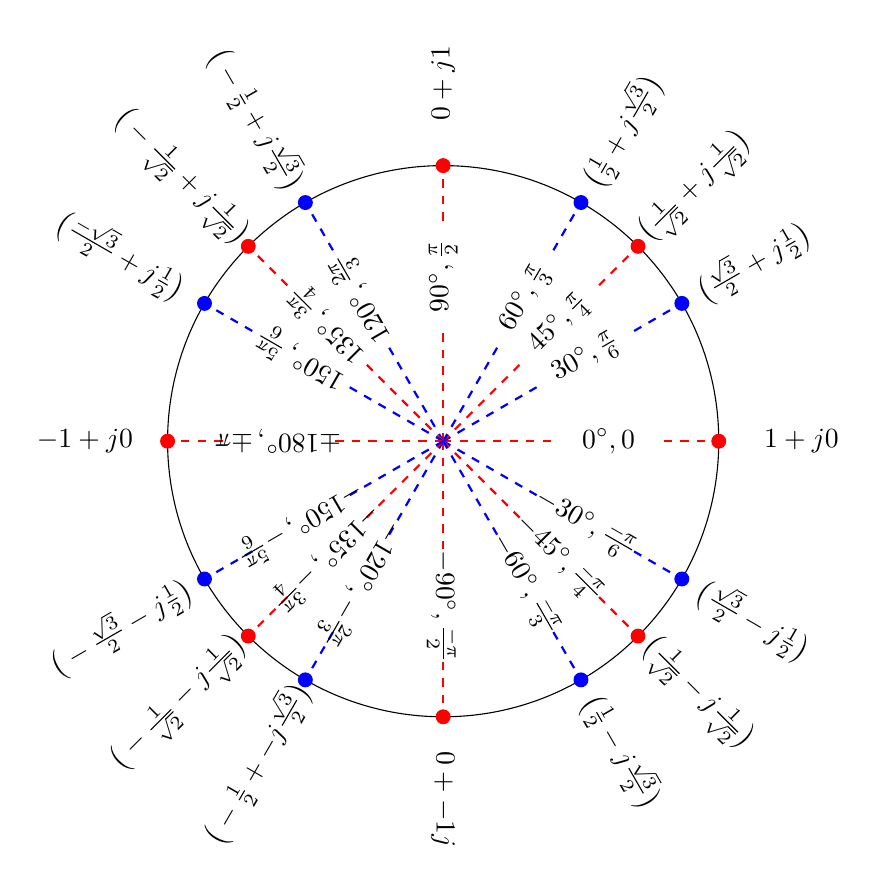
\begin{tikzpicture}[scale=0.7]
%\draw[style=help lines] (-12,-12) grid (12,12);
%\draw[black,->] (-12,0) -- (12,0);
%\draw[black,->] (0,-12) -- (0,12);

\draw (0,0) circle[radius=5];

\draw[fill,red] (0:5cm) circle[radius=0.125];
\draw[red,dashed,thick] (0,0) -- (0:2cm) (0:4cm) -- (0:5cm);
\node[rotate=0] at (0:3cm){$0^\circ, 0$};
\node at (0:6.5cm)[rotate=0]{$1+j0$};

\draw[fill,blue] (30:5cm) circle[radius=0.125];
\draw[blue,dashed,thick] (0,0) -- (30:2cm) (30:4cm) -- (30:5cm);
\node[rotate=30] at (30:3cm){$30^\circ, \frac{\pi}{6}$};
\node at (30:6.5cm)[rotate=30]{$\big(\frac{\sqrt{3}}{2}+j\frac{1}{2} \big)$};

\draw[fill,red] (45:5cm) circle[radius=0.125];
\draw[red,dashed,thick] (0,0) -- (45:2cm) (45:4cm) -- (45:5cm);
\node[rotate=45] at (45:3cm){$45^\circ, \frac{\pi}{4}$};
\node at (45:6.5cm)[rotate=45]{$\big(\frac{1}{\sqrt{2}}+j\frac{1}{\sqrt{2}} \big)$};

\draw[fill,blue] (60:5cm) circle[radius=0.125];
\draw[blue,dashed,thick] (0,0) -- (60:2cm) (60:4cm) -- (60:5cm);
\node[rotate=60] at (60:3cm){$60^\circ, \frac{\pi}{3}$};
\node at (60:6.5cm)[rotate=60]{$\big(\frac{1}{2}+j\frac{\sqrt{3}}{2} \big)$};

\draw[fill,red] (90:5cm) circle[radius=0.125];
\draw[red,dashed,thick] (0,0) -- (90:2cm) (90:4cm) -- (90:5cm);
\node[rotate=90] at (90:3cm){$90^\circ, \frac{\pi}{2}$};
\node at (90:6.5cm)[rotate=90]{$0+j1$};

\draw[fill,blue] (120:5cm) circle[radius=0.125];
\draw[blue,dashed,thick] (0,0) -- (120:2cm) (120:4cm) -- (120:5cm);
\node[rotate=120] at (120:3cm){$120^\circ, \frac{2\pi}{3}$};
\node at (120:6.75cm)[rotate=-60]{$\big(-\frac{1}{2}+j\frac{\sqrt{3}}{2} \big)$};

\draw[fill,red] (135:5cm) circle[radius=0.125];
\draw[red,dashed,thick] (0,0) -- (135:2cm) (135:4cm) -- (135:5cm);
\node[rotate=135] at (135:3cm){$135^\circ, \frac{3\pi}{4}$};
\node at (135:6.75cm)[rotate=-45]{$\big(-\frac{1}{\sqrt{2}}+j\frac{1}{\sqrt{2}} \big)$};

\draw[fill,blue] (150:5cm) circle[radius=0.125];
\draw[blue,dashed,thick] (0,0) -- (150:2cm) (150:4cm) -- (150:5cm);
\node[rotate=150] at (150:3cm){$150^\circ, \frac{5\pi}{6}$};
\node at (150:6.75cm)[rotate=-30]{$\big(\frac{-\sqrt{3}}{2}+j\frac{1}{2} \big)$};

R\draw[fill,red] (180:5cm) circle[radius=0.125];
\draw[red,dashed,thick] (0,0) -- (180:2cm) (180:4cm) -- (180:5cm);
\node[rotate=180] at (180:3cm){$\pm 180^\circ, \pm \pi$};
\node at (180:6.5cm)[rotate=0]{$-1+j0$};

\draw[fill,blue] (-30:5cm) circle[radius=0.125];
\draw[blue,dashed,thick] (0,0) -- (-30:2cm) (-30:4cm) -- (-30:5cm);
\node[rotate=-30] at (-30:3cm){$-30^\circ, \frac{-\pi}{6}$};
\node at (-30:6.5cm)[rotate=-30]{$\big(\frac{\sqrt{3}}{2}-j\frac{1}{2} \big)$};

\draw[fill,red] (-45:5cm) circle[radius=0.125];
\draw[red,dashed,thick] (0,0) -- (-45:2cm) (-45:4cm) -- (-45:5cm);
\node[rotate=-45] at (-45:3cm){$-45^\circ, \frac{-\pi}{4}$};
\node at (-45:6.5cm)[rotate=-45]{$\big(\frac{1}{\sqrt{2}}-j\frac{1}{\sqrt{2}} \big)$};

\draw[fill,blue] (-60:5cm) circle[radius=0.125];
\draw[blue,dashed,thick] (0,0) -- (-60:2cm) (-60:4cm) -- (-60:5cm);
\node[rotate=-60] at (-60:3cm){$-60^\circ, \frac{-\pi}{3}$};
\node at (-60:6.5cm)[rotate=-60]{$\big(\frac{1}{2}-j\frac{\sqrt{3}}{2} \big)$};

\draw[fill,red] (-90:5cm) circle[radius=0.125];
\draw[red,dashed,thick] (0,0) -- (-90:2cm) (-90:4cm) -- (-90:5cm);
\node[rotate=-90] at (-90:3cm){$-90^\circ, \frac{-\pi}{2}$};
\node at (-90:6.5cm)[rotate=-90]{$0+-1j$};

\draw[fill,blue] (-120:5cm) circle[radius=0.125];
\draw[blue,dashed,thick] (0,0) -- (-120:2cm) (-120:4cm) -- (-120:5cm);
\node[rotate=-120] at (-120:3cm){$-120^\circ, -\frac{2\pi}{3}$};
\node at (-120:6.75cm)[rotate=60]{$\big(-\frac{1}{2}+-j\frac{\sqrt{3}}{2} \big)$};

\draw[fill,red] (-135:5cm) circle[radius=0.125];
\draw[red,dashed,thick] (0,0) -- (-135:2cm) (-135:4cm) -- (-135:5cm);
\node[rotate=-135] at (-135:3cm){$-135^\circ, -\frac{3\pi}{4}$};
\node at (-135:6.75cm)[rotate=45]{$\big(-\frac{1}{\sqrt{2}}-j\frac{1}{\sqrt{2}} \big)$};

\draw[fill,blue] (-150:5cm) circle[radius=0.125];
\draw[blue,dashed,thick] (0,0) -- (-150:2cm) (-150:4cm) -- (-150:5cm);
\node[rotate=-150] at (-150:3cm){$-150^\circ,-\frac{5\pi}{6}$};
%\node[rotate=-150] at (-150:3.5cm){$-\frac{\pi}{6}$};
\node at (-150:6.75cm)[rotate=30]{$\big(-\frac{\sqrt{3}}{2}-j\frac{1}{2} \big)$};

\end{tikzpicture}
%\end{document} 